% Options for packages loaded elsewhere
\PassOptionsToPackage{unicode}{hyperref}
\PassOptionsToPackage{hyphens}{url}
%
\documentclass[
]{article}
\usepackage{lmodern}
\usepackage{amssymb,amsmath}
\usepackage{ifxetex,ifluatex}
\ifnum 0\ifxetex 1\fi\ifluatex 1\fi=0 % if pdftex
  \usepackage[T1]{fontenc}
  \usepackage[utf8]{inputenc}
  \usepackage{textcomp} % provide euro and other symbols
\else % if luatex or xetex
  \usepackage{unicode-math}
  \defaultfontfeatures{Scale=MatchLowercase}
  \defaultfontfeatures[\rmfamily]{Ligatures=TeX,Scale=1}
\fi
% Use upquote if available, for straight quotes in verbatim environments
\IfFileExists{upquote.sty}{\usepackage{upquote}}{}
\IfFileExists{microtype.sty}{% use microtype if available
  \usepackage[]{microtype}
  \UseMicrotypeSet[protrusion]{basicmath} % disable protrusion for tt fonts
}{}
\makeatletter
\@ifundefined{KOMAClassName}{% if non-KOMA class
  \IfFileExists{parskip.sty}{%
    \usepackage{parskip}
  }{% else
    \setlength{\parindent}{0pt}
    \setlength{\parskip}{6pt plus 2pt minus 1pt}}
}{% if KOMA class
  \KOMAoptions{parskip=half}}
\makeatother
\usepackage{xcolor}
\IfFileExists{xurl.sty}{\usepackage{xurl}}{} % add URL line breaks if available
\IfFileExists{bookmark.sty}{\usepackage{bookmark}}{\usepackage{hyperref}}
\hypersetup{
  pdftitle={Results of Ordered Likelihood Analysis},
  pdfauthor={Devan Becker},
  hidelinks,
  pdfcreator={LaTeX via pandoc}}
\urlstyle{same} % disable monospaced font for URLs
\usepackage[margin=1in]{geometry}
\usepackage{color}
\usepackage{fancyvrb}
\newcommand{\VerbBar}{|}
\newcommand{\VERB}{\Verb[commandchars=\\\{\}]}
\DefineVerbatimEnvironment{Highlighting}{Verbatim}{commandchars=\\\{\}}
% Add ',fontsize=\small' for more characters per line
\usepackage{framed}
\definecolor{shadecolor}{RGB}{248,248,248}
\newenvironment{Shaded}{\begin{snugshade}}{\end{snugshade}}
\newcommand{\AlertTok}[1]{\textcolor[rgb]{0.94,0.16,0.16}{#1}}
\newcommand{\AnnotationTok}[1]{\textcolor[rgb]{0.56,0.35,0.01}{\textbf{\textit{#1}}}}
\newcommand{\AttributeTok}[1]{\textcolor[rgb]{0.77,0.63,0.00}{#1}}
\newcommand{\BaseNTok}[1]{\textcolor[rgb]{0.00,0.00,0.81}{#1}}
\newcommand{\BuiltInTok}[1]{#1}
\newcommand{\CharTok}[1]{\textcolor[rgb]{0.31,0.60,0.02}{#1}}
\newcommand{\CommentTok}[1]{\textcolor[rgb]{0.56,0.35,0.01}{\textit{#1}}}
\newcommand{\CommentVarTok}[1]{\textcolor[rgb]{0.56,0.35,0.01}{\textbf{\textit{#1}}}}
\newcommand{\ConstantTok}[1]{\textcolor[rgb]{0.00,0.00,0.00}{#1}}
\newcommand{\ControlFlowTok}[1]{\textcolor[rgb]{0.13,0.29,0.53}{\textbf{#1}}}
\newcommand{\DataTypeTok}[1]{\textcolor[rgb]{0.13,0.29,0.53}{#1}}
\newcommand{\DecValTok}[1]{\textcolor[rgb]{0.00,0.00,0.81}{#1}}
\newcommand{\DocumentationTok}[1]{\textcolor[rgb]{0.56,0.35,0.01}{\textbf{\textit{#1}}}}
\newcommand{\ErrorTok}[1]{\textcolor[rgb]{0.64,0.00,0.00}{\textbf{#1}}}
\newcommand{\ExtensionTok}[1]{#1}
\newcommand{\FloatTok}[1]{\textcolor[rgb]{0.00,0.00,0.81}{#1}}
\newcommand{\FunctionTok}[1]{\textcolor[rgb]{0.00,0.00,0.00}{#1}}
\newcommand{\ImportTok}[1]{#1}
\newcommand{\InformationTok}[1]{\textcolor[rgb]{0.56,0.35,0.01}{\textbf{\textit{#1}}}}
\newcommand{\KeywordTok}[1]{\textcolor[rgb]{0.13,0.29,0.53}{\textbf{#1}}}
\newcommand{\NormalTok}[1]{#1}
\newcommand{\OperatorTok}[1]{\textcolor[rgb]{0.81,0.36,0.00}{\textbf{#1}}}
\newcommand{\OtherTok}[1]{\textcolor[rgb]{0.56,0.35,0.01}{#1}}
\newcommand{\PreprocessorTok}[1]{\textcolor[rgb]{0.56,0.35,0.01}{\textit{#1}}}
\newcommand{\RegionMarkerTok}[1]{#1}
\newcommand{\SpecialCharTok}[1]{\textcolor[rgb]{0.00,0.00,0.00}{#1}}
\newcommand{\SpecialStringTok}[1]{\textcolor[rgb]{0.31,0.60,0.02}{#1}}
\newcommand{\StringTok}[1]{\textcolor[rgb]{0.31,0.60,0.02}{#1}}
\newcommand{\VariableTok}[1]{\textcolor[rgb]{0.00,0.00,0.00}{#1}}
\newcommand{\VerbatimStringTok}[1]{\textcolor[rgb]{0.31,0.60,0.02}{#1}}
\newcommand{\WarningTok}[1]{\textcolor[rgb]{0.56,0.35,0.01}{\textbf{\textit{#1}}}}
\usepackage{graphicx}
\makeatletter
\def\maxwidth{\ifdim\Gin@nat@width>\linewidth\linewidth\else\Gin@nat@width\fi}
\def\maxheight{\ifdim\Gin@nat@height>\textheight\textheight\else\Gin@nat@height\fi}
\makeatother
% Scale images if necessary, so that they will not overflow the page
% margins by default, and it is still possible to overwrite the defaults
% using explicit options in \includegraphics[width, height, ...]{}
\setkeys{Gin}{width=\maxwidth,height=\maxheight,keepaspectratio}
% Set default figure placement to htbp
\makeatletter
\def\fps@figure{htbp}
\makeatother
\setlength{\emergencystretch}{3em} % prevent overfull lines
\providecommand{\tightlist}{%
  \setlength{\itemsep}{0pt}\setlength{\parskip}{0pt}}
\setcounter{secnumdepth}{-\maxdimen} % remove section numbering
\usepackage[]{natbib}
\bibliographystyle{plainnat}

\title{Results of Ordered Likelihood Analysis}
\author{Devan Becker}
\date{2021-04-14}

\begin{document}
\maketitle

\begin{Shaded}
\begin{Highlighting}[]
\KeywordTok{library}\NormalTok{(here)}
\KeywordTok{library}\NormalTok{(dplyr)}
\KeywordTok{library}\NormalTok{(tidyr)}
\KeywordTok{library}\NormalTok{(stringr)}
\KeywordTok{library}\NormalTok{(ggplot2)}
\NormalTok{ords \textless{}{-}}\StringTok{ }\KeywordTok{lapply}\NormalTok{(}
    \KeywordTok{list.files}\NormalTok{(}\KeywordTok{here}\NormalTok{(}\StringTok{"data/pangordlineages"}\NormalTok{),}
        \DataTypeTok{full.names =} \OtherTok{TRUE}\NormalTok{),}
\NormalTok{    read.csv}
\NormalTok{    ) }\OperatorTok{\%\textgreater{}\%}
\StringTok{    }\KeywordTok{bind\_rows}\NormalTok{() }\OperatorTok{\%\textgreater{}\%}
\StringTok{    }\KeywordTok{separate}\NormalTok{(}\DataTypeTok{col =}\NormalTok{ taxon, }
        \DataTypeTok{into =} \KeywordTok{c}\NormalTok{(}\StringTok{"dummy"}\NormalTok{, }\StringTok{"acc"}\NormalTok{, }\StringTok{"lik"}\NormalTok{, }\StringTok{"subs"}\NormalTok{),}
        \DataTypeTok{sep =} \StringTok{"\_"}\NormalTok{) }\OperatorTok{\%\textgreater{}\%}
\StringTok{    }\KeywordTok{mutate}\NormalTok{(}\DataTypeTok{nsubs =} \KeywordTok{str\_count}\NormalTok{(subs, }\StringTok{"2"}\NormalTok{),}
        \DataTypeTok{lik =} \KeywordTok{as.numeric}\NormalTok{(lik)) }\OperatorTok{\%\textgreater{}\%}
\StringTok{    }\KeywordTok{group\_by}\NormalTok{(acc) }\OperatorTok{\%\textgreater{}\%}
\StringTok{    }\KeywordTok{mutate}\NormalTok{(}\DataTypeTok{order =} \DecValTok{1}\OperatorTok{:}\KeywordTok{n}\NormalTok{()) }\OperatorTok{\%\textgreater{}\%}
\StringTok{    }\KeywordTok{ungroup}\NormalTok{()}
\end{Highlighting}
\end{Shaded}

\begin{Shaded}
\begin{Highlighting}[]
\KeywordTok{ggplot}\NormalTok{(}\KeywordTok{filter}\NormalTok{(ords, order }\OperatorTok{\textless{}}\StringTok{ }\DecValTok{1024}\NormalTok{)) }\OperatorTok{+}
\StringTok{    }\KeywordTok{aes}\NormalTok{(}\DataTypeTok{x =}\NormalTok{ order, }\DataTypeTok{y =}\NormalTok{ lik, }\DataTypeTok{colour =} \KeywordTok{factor}\NormalTok{(acc)) }\OperatorTok{+}\StringTok{ }
\StringTok{    }\KeywordTok{geom\_line}\NormalTok{() }\OperatorTok{+}
\StringTok{    }\KeywordTok{theme}\NormalTok{(}\DataTypeTok{legend.position =} \StringTok{"none"}\NormalTok{)}
\end{Highlighting}
\end{Shaded}

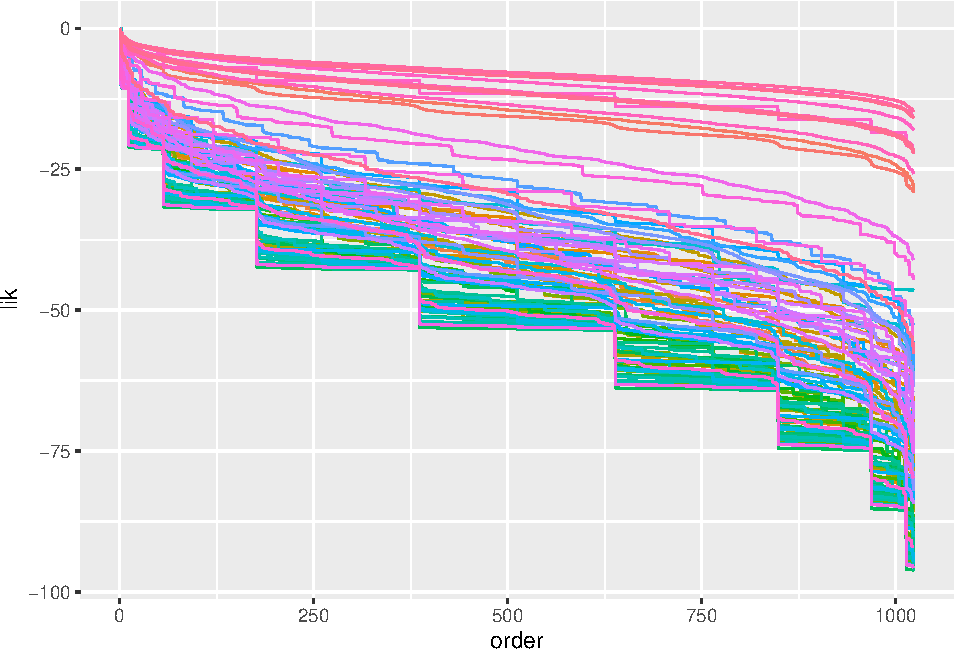
\includegraphics{ord-results_files/figure-latex/change_in_weight-1.pdf}

\begin{Shaded}
\begin{Highlighting}[]
\NormalTok{ords }\OperatorTok{\%\textgreater{}\%}
\StringTok{    }\KeywordTok{group\_by}\NormalTok{(acc) }\OperatorTok{\%\textgreater{}\%}
\StringTok{    }\KeywordTok{summarise}\NormalTok{(}\DataTypeTok{unique =} \KeywordTok{length}\NormalTok{(}\KeywordTok{unique}\NormalTok{(lineage))) }\OperatorTok{\%\textgreater{}\%}
\StringTok{    }\KeywordTok{print}\NormalTok{(}\DataTypeTok{n =} \OtherTok{Inf}\NormalTok{)}
\end{Highlighting}
\end{Shaded}

\begin{verbatim}
## `summarise()` ungrouping output (override with `.groups` argument)
\end{verbatim}

\begin{verbatim}
## # A tibble: 100 x 2
##     acc         unique
##     <chr>        <int>
##   1 ERR4085809       1
##   2 ERR4204823       1
##   3 ERR4305816       1
##   4 ERR4307842       1
##   5 ERR4363387       1
##   6 ERR4364007       1
##   7 ERR4667618       1
##   8 ERR4692364       1
##   9 ERR4693034       1
##  10 ERR4693061       1
##  11 ERR4693079       1
##  12 ERR4693537       1
##  13 ERR4759453       1
##  14 ERR4869446       1
##  15 ERR4869458       1
##  16 ERR4869480       1
##  17 ERR4869487       1
##  18 ERR4869497       1
##  19 ERR4891711       1
##  20 ERR4891715       1
##  21 ERR4891805       1
##  22 ERR4891841       1
##  23 ERR4891863       1
##  24 ERR4891889       1
##  25 ERR4891898       1
##  26 ERR4891916       1
##  27 ERR4891988       1
##  28 ERR4892048       1
##  29 ERR4892066       1
##  30 ERR4892112       1
##  31 ERR4892152       1
##  32 ERR4892200       1
##  33 ERR4892203       1
##  34 ERR4892293       1
##  35 ERR4892339       1
##  36 ERR4892386       1
##  37 ERR4892392       1
##  38 ERR4892423       1
##  39 ERR4893013       1
##  40 ERR4893031       1
##  41 ERR4893033       1
##  42 ERR4893037       1
##  43 ERR4893080       1
##  44 ERR4893138       1
##  45 ERR4893184       1
##  46 ERR4893186       1
##  47 ERR4893197       1
##  48 ERR4893242       1
##  49 ERR4893353       1
##  50 ERR4893393       1
##  51 ERR4999251       1
##  52 ERR4999255       1
##  53 ERR4999275       1
##  54 ERR4999282       1
##  55 ERR5062571       1
##  56 ERR5063165       1
##  57 ERR5064166       1
##  58 ERR5069584       1
##  59 ERR5069616       1
##  60 ERR5069624       1
##  61 ERR5069871       1
##  62 ERR5070060       1
##  63 ERR5070294       1
##  64 ERR5074314       1
##  65 ERR5076163       1
##  66 ERR5076748       1
##  67 ERR5077151       1
##  68 ERR5077411       1
##  69 ERR5077618       1
##  70 ERR5080893       1
##  71 ERR5080897       1
##  72 ERR5080913       1
##  73 ERR5080918       1
##  74 ERR5081301       1
##  75 ERR5081316       1
##  76 ERR5082556       1
##  77 ERR5082569       1
##  78 ERR5082580       1
##  79 ERR5082590       1
##  80 ERR5082610       1
##  81 ERR5082630       1
##  82 ERR5082645       1
##  83 ERR5082664       1
##  84 ERR5082695       1
##  85 ERR5082696       1
##  86 ERR5082711       1
##  87 ERR5082712       1
##  88 SRR12639958      1
##  89 SRR12762573      1
##  90 SRR13020989      1
##  91 SRR13020990      1
##  92 SRR13021027      1
##  93 SRR13021032      1
##  94 SRR13021033      1
##  95 SRR13021035      1
##  96 SRR13021038      1
##  97 SRR13021042      1
##  98 SRR13021047      1
##  99 SRR13021097      1
## 100 SRR13092002      1
\end{verbatim}

\end{document}
